\documentclass{article}
\usepackage{graphicx}
\usepackage[utf8]{inputenc}

\title{Compte rendu Pilotage, réunion du 9 Avril}
\author{Johan Rossi, Qingyuan Yao}

\date{April 10 2021}

\begin{document}

\maketitle

\section{Architecture:}
\begin{itemize}
    \item Fixer définitivement les variables d'interface entre les parties dans le commun.h (décision/Pilotage ...)
\end{itemize}

\begin{figure}[h]
\caption{Schéma de l'architecture du projet}
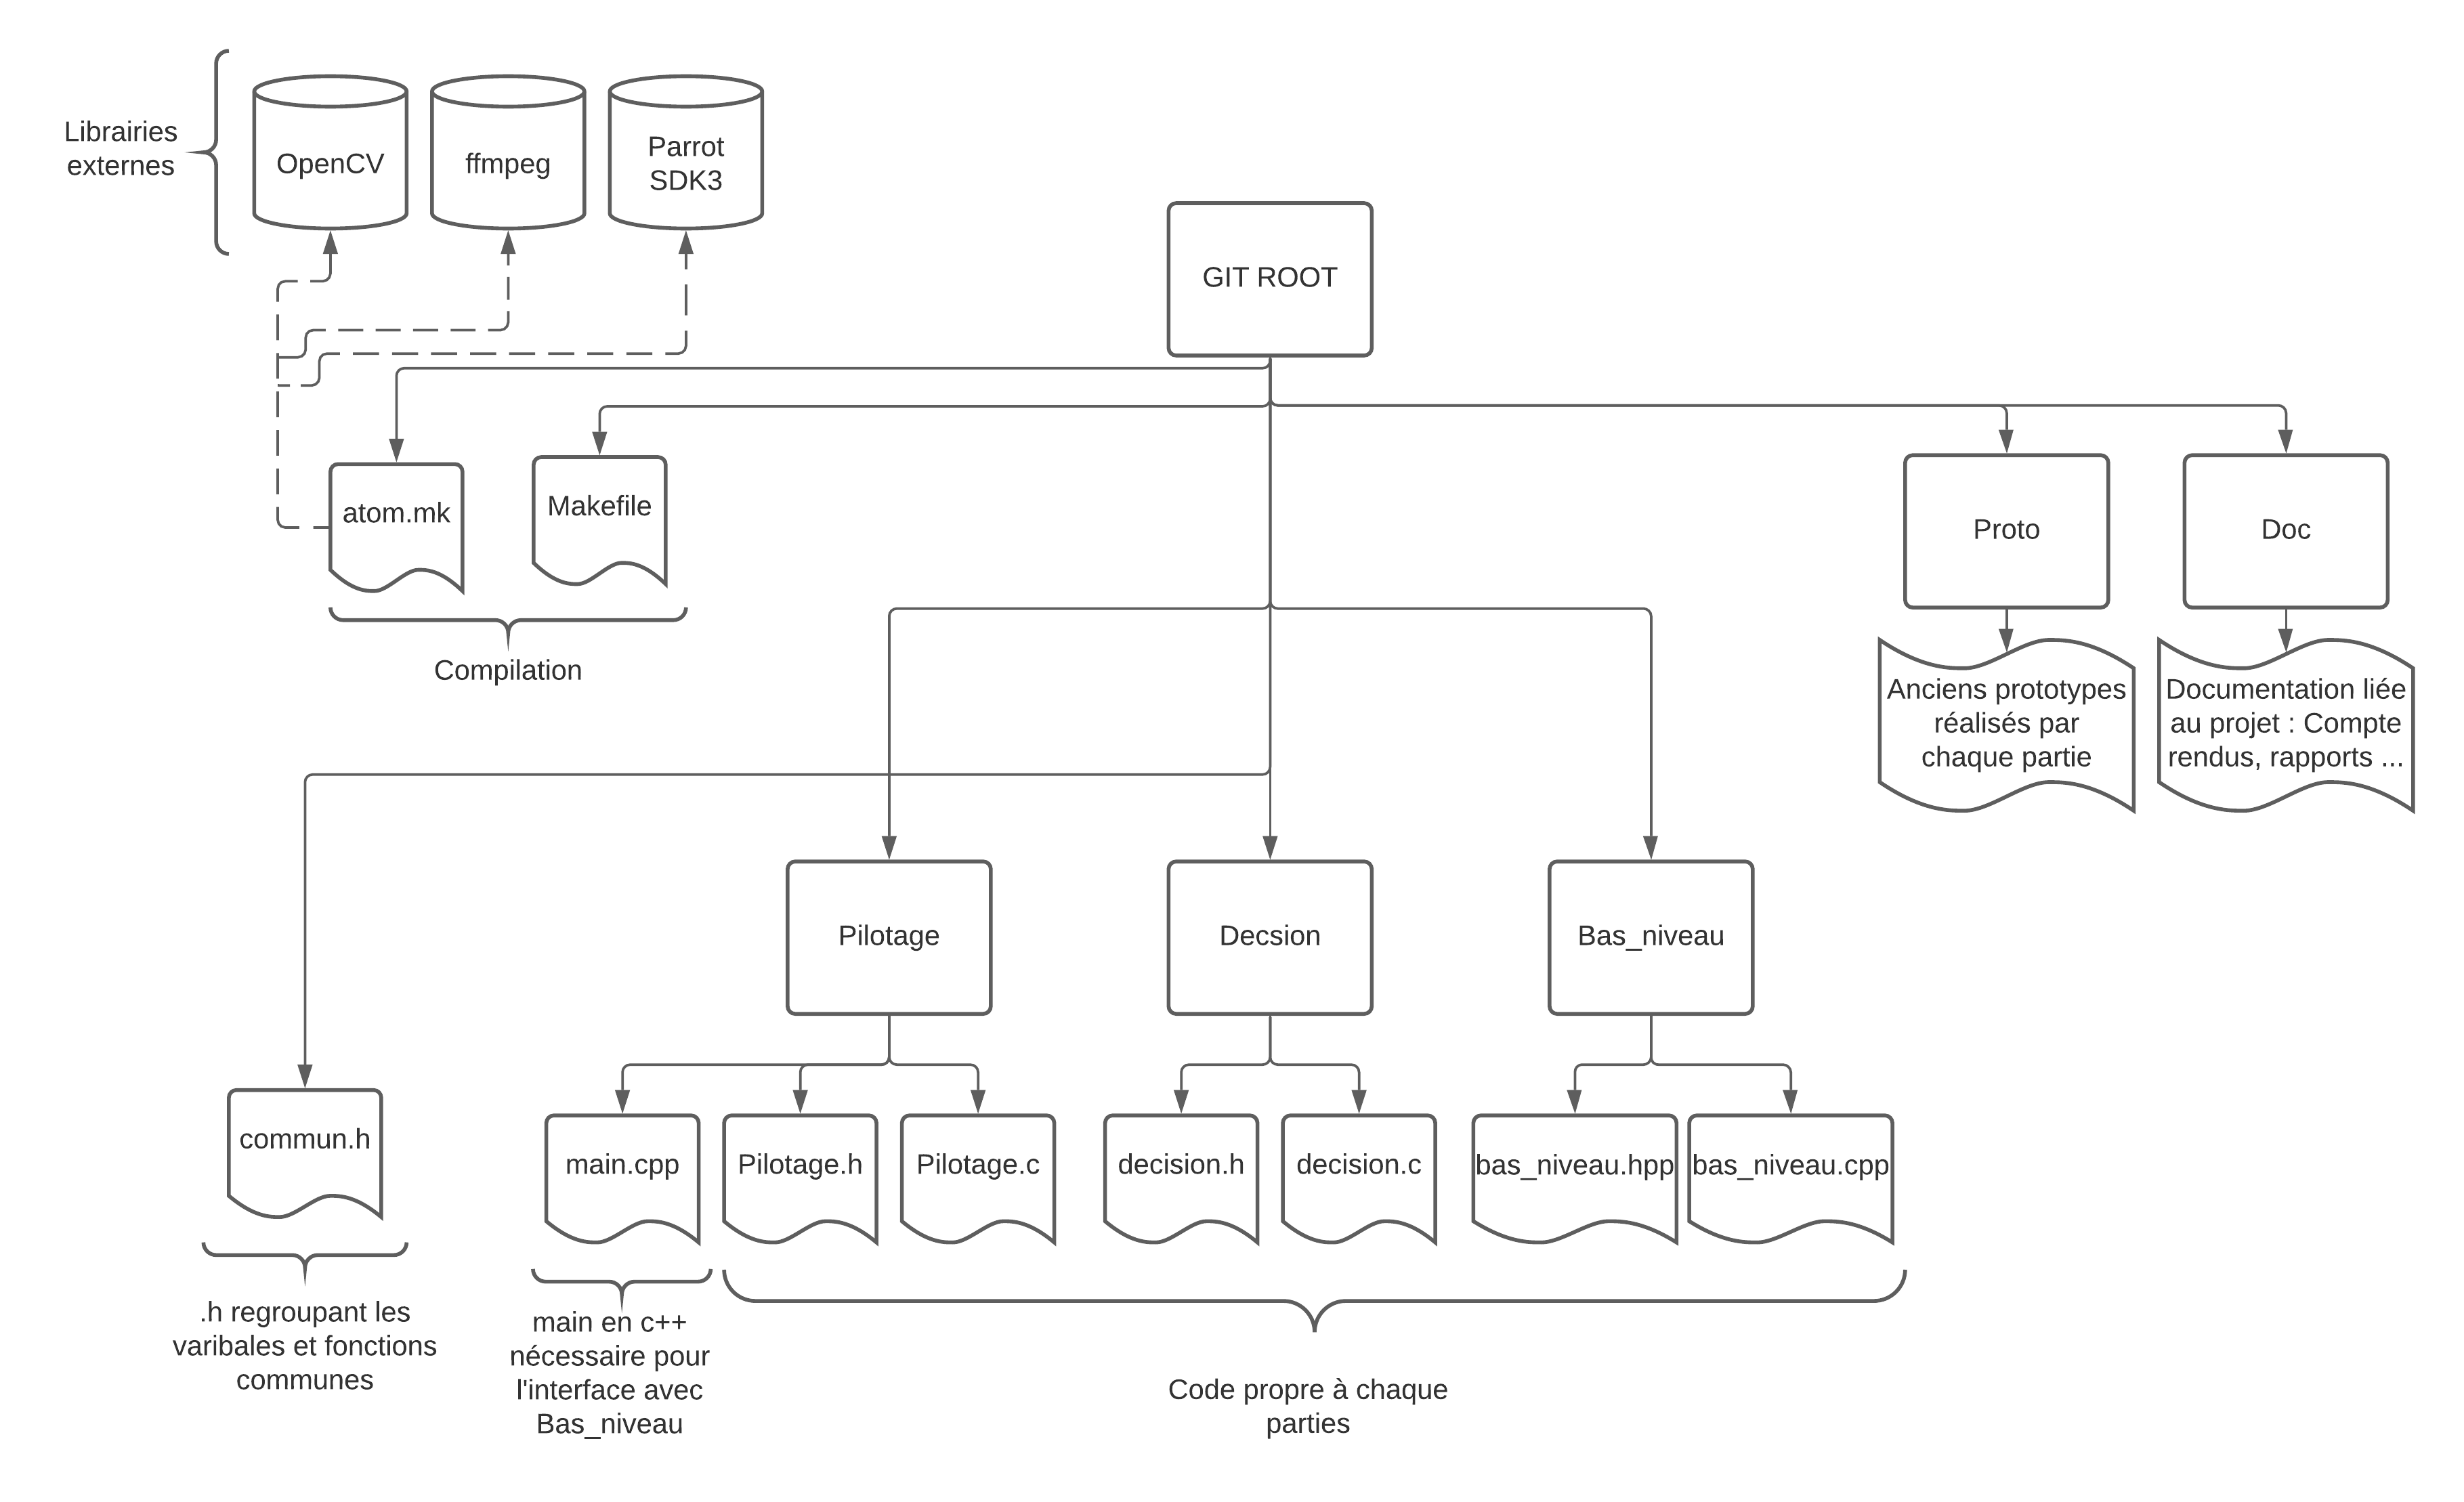
\includegraphics[scale=0.5]{Architecture projet Drone (1).png}
\centering
\end{figure}

\section{Création de bouchons}
\begin{itemize}
    \item Continuer la création de bouchons avec les nouvelles interfaces (matrice 4x3 de la partie décision) et commencer a tester les mécanisme de conservation du drone (watchdog ...).
\end{itemize}

\section{Watchdog, récupération des signaux, exceptions ...}
\begin{itemize}
    \item Implémenter le Test\_Watchdog.c dans Pilotage.c
    \item Attraper tous les signaux possibles qui peuvent crasher le programme
    \item Tester le watchdog dans le simulateur
    \item Gérer les exception venant de la partie C++ du projet (BasNiveau).
\end{itemize}


\end{document}
